\documentclass[12pt]{article}
\usepackage{graphicx}
\usepackage{listings}
\usepackage{xcolor}
\usepackage{circuitikz}

\definecolor{codegreen}{rgb}{0,0.6,0}
\definecolor{codegray}{rgb}{0.5,0.5,0.5}
\definecolor{codepurple}{rgb}{0.58,0,0.82}
\definecolor{backcolour}{rgb}{0.95,0.95,0.92}

\lstdefinelanguage{SPICE}{
  keywords={.dc, .meas},
  morecomment=[l]{*},
  morecomment=[l]{\$}
  morecomment=[s]{/*}{*/},
  morestring=[b]',
  morestring=[b]",
  ndkeywords={.tran, .ac, boolean, throw, implements, import, this},
  keywordstyle=\color{blue}\bfseries,
  ndkeywordstyle=\color{darkgray}\bfseries,
  identifierstyle=\color{black},
  commentstyle=\color{purple}\ttfamily,
  stringstyle=\color{red}\ttfamily,
  sensitive=true
}

\lstdefinestyle{mystyle}{
	backgroundcolor=\color{backcolour},   
    commentstyle=\color{codegreen},
    keywordstyle=\color{magenta},
    numberstyle=\tiny\color{codegray},
    stringstyle=\color{codepurple},
    basicstyle=\ttfamily\footnotesize,
    breakatwhitespace=false,         
    breaklines=true,                 
    captionpos=b,                    
    keepspaces=true,                 
    numbers=left,                    
    numbersep=5pt,                  
    showspaces=false,                
    showstringspaces=false,
    showtabs=false,                  
    tabsize=4
}

\lstset{style=mystyle}

% Title[Enter title of the experiment here]
\title{EE230: Homework-1\\
Familiarization with NGSPICE Circuit Simulator and Lab Equipment}

% Author[Enter details of author here]
\author{Prateek Garg, 20D070060}

% begin the document.
\begin{document}
\noindent
% make a title page.[this creates title page]
\maketitle

\section{Overview of the experiment} %[This segment creates Section as seen in document]

\subsection{Aim of the experiment}%[This segment creates sebsections under the same section]

Ngspice is a mixed-signal circuit Simulator. This experiment aims to implement some basic circuits namely :
\begin{itemize}
	\item RC Integrator
	\item RC Differentiator
	\item RC Lowpass Filter
	\item RC Highpass Filter
	\item RC Bandpass Filter
	\item RLC Bandpass Filter
\end{itemize}
in Ngspice and plot their characteristics.

\subsection{Methods}

We start by creating a netlist for each circuit, simulating on Ngspice and exporting the values to a python script to plot them using Matplotlib.
\section{Design}
%Add circuit Diagrams here
%With accompaying Explanantions 
<<<<<<< HEAD
% XCircuit output "RC_Integrator.eps.tex" for LaTeX input from RC_Integrator.eps.ps
\def\putbox#1#2#3{\makebox[0in][l]{\makebox[#1][l]{}\raisebox{\baselineskip}[0in][0in]{\raisebox{#2}[0in][0in]{#3}}}}
\def\rightbox#1{\makebox[0in][r]{#1}}
\def\centbox#1{\makebox[0in]{#1}}
\def\topbox#1{\raisebox{-\baselineskip}[0in][0in]{#1}}
\def\midbox#1{\raisebox{-0.5\baselineskip}[0in][0in]{#1}}
\begin{flushleft}
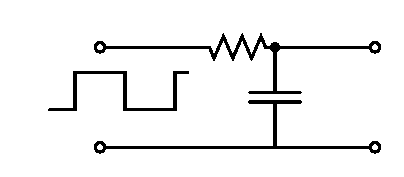
\includegraphics[width=\textwidth]{RC_Integrator.eps}\\
% translate x=624 y=118 scale 0.38
\putbox{1.31in}{0.84in}{R=10K$\Omega$}%
\putbox{1.81in}{0.25in}{C=0.1$\mu$F}%
\putbox{0.06in}{0.42in}{$V_{in}$}%
\putbox{0.47in}{0.50in}{5v}%
\putbox{0.89in}{0.25in}{0v}%
\end{flushleft}
=======
\begin{center}
    \begin{circuitikz}[american voltages]
        \draw
        (0,0) to [short, o-o] (6,0)
        to [open, v>=$V_{out}$] (6,4) 
        (0,0) to [open, v^>=$V_{in}$,o-o] (0,4)  
        to [R, l= $10K \Omega $,o-o] (6,4)
        (5,4) to [C, l_=$0.1\mu F$,*-*] (5,0); 
    \end{circuitikz}

    RC Integrator Circuit
\end{center}

>>>>>>> circuitikz

\section{Simulation results}

\subsection{RC Integrator}
\subsubsection{Code snippet}
\lstinputlisting[language=SPICE]{../RC_Integrator.cir}
\subsubsection{Simulation results}
\makebox[\textwidth]{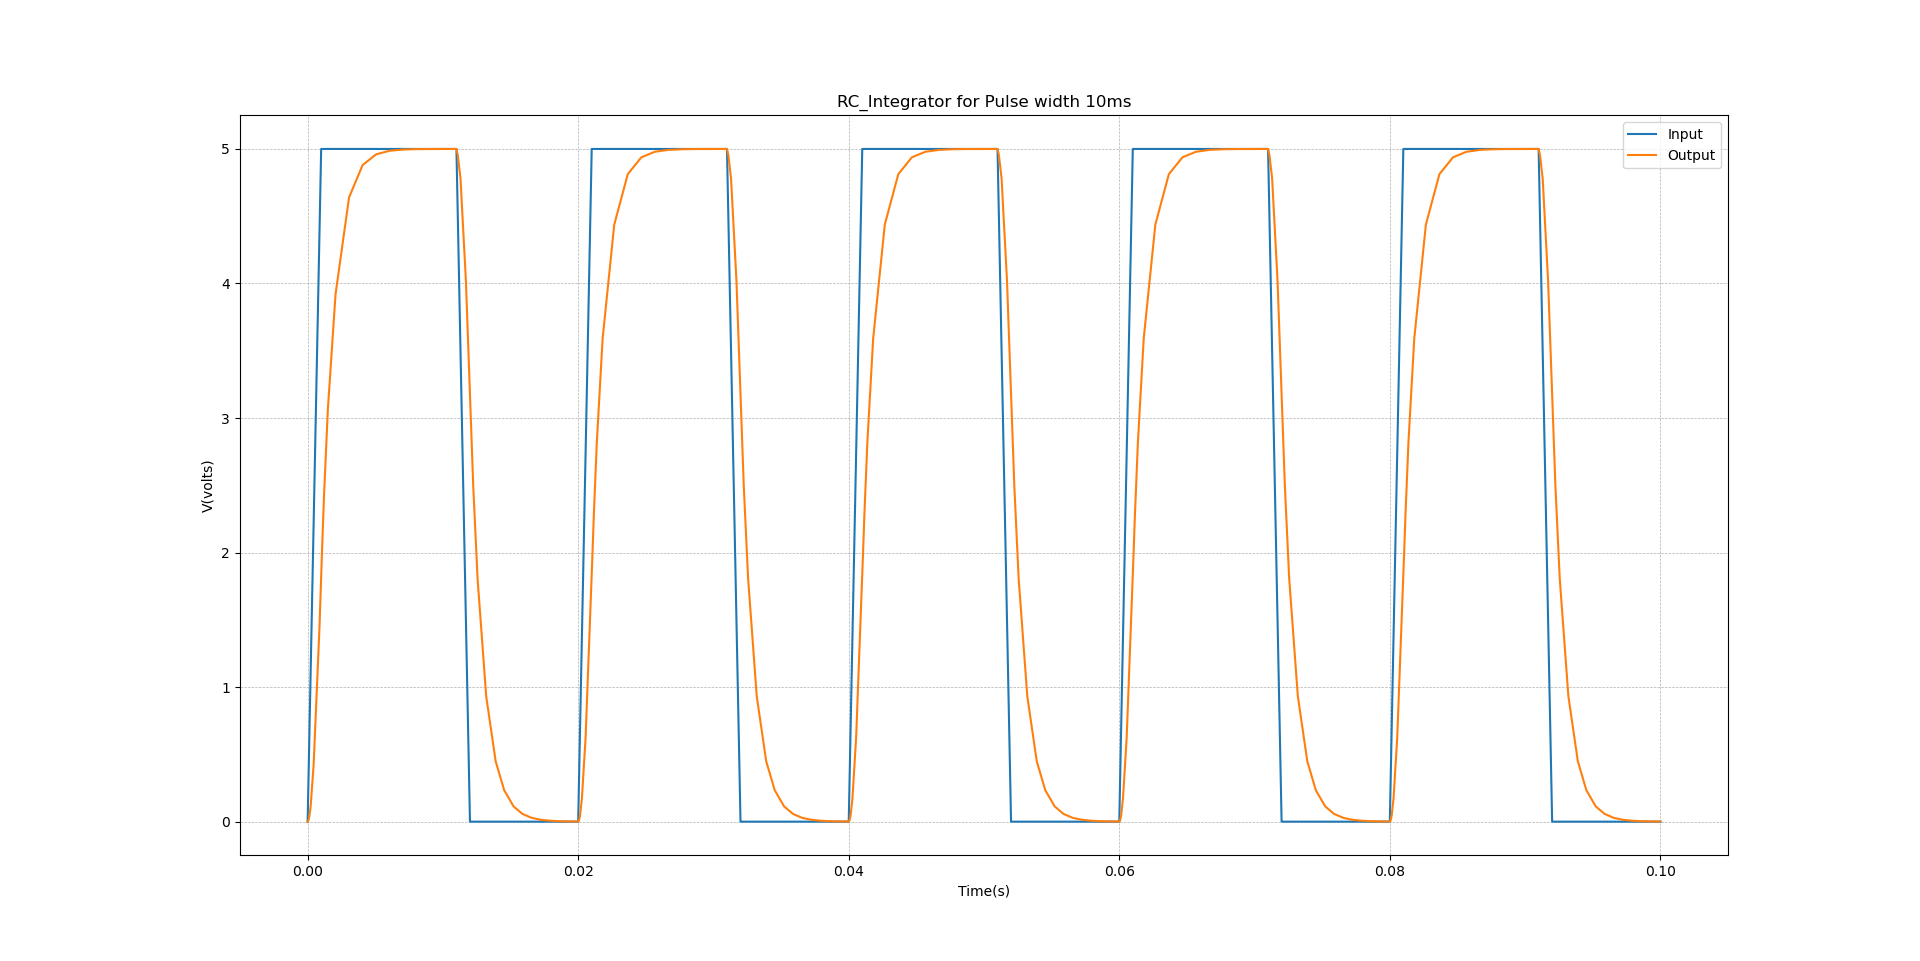
\includegraphics[width=\paperwidth]{RC_Integrator_1.png}}
\makebox[\textwidth]{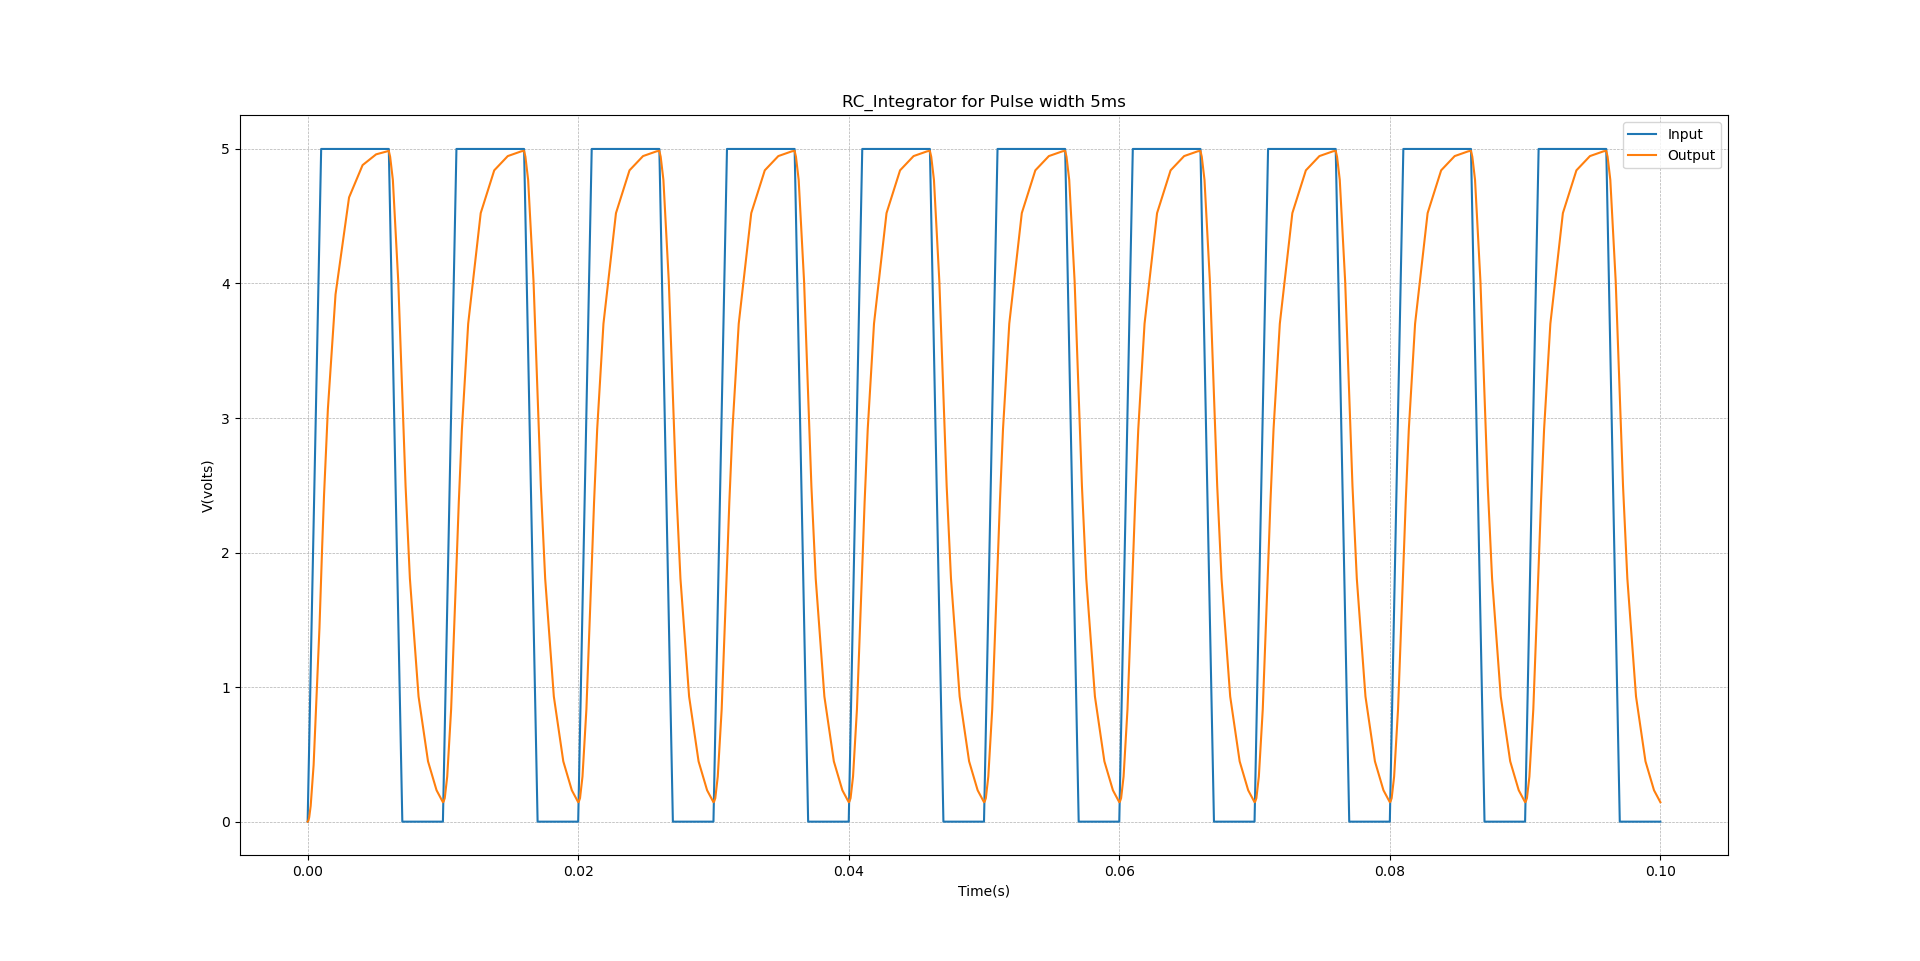
\includegraphics[width=\paperwidth]{RC_Integrator_2.png}}
\makebox[\textwidth]{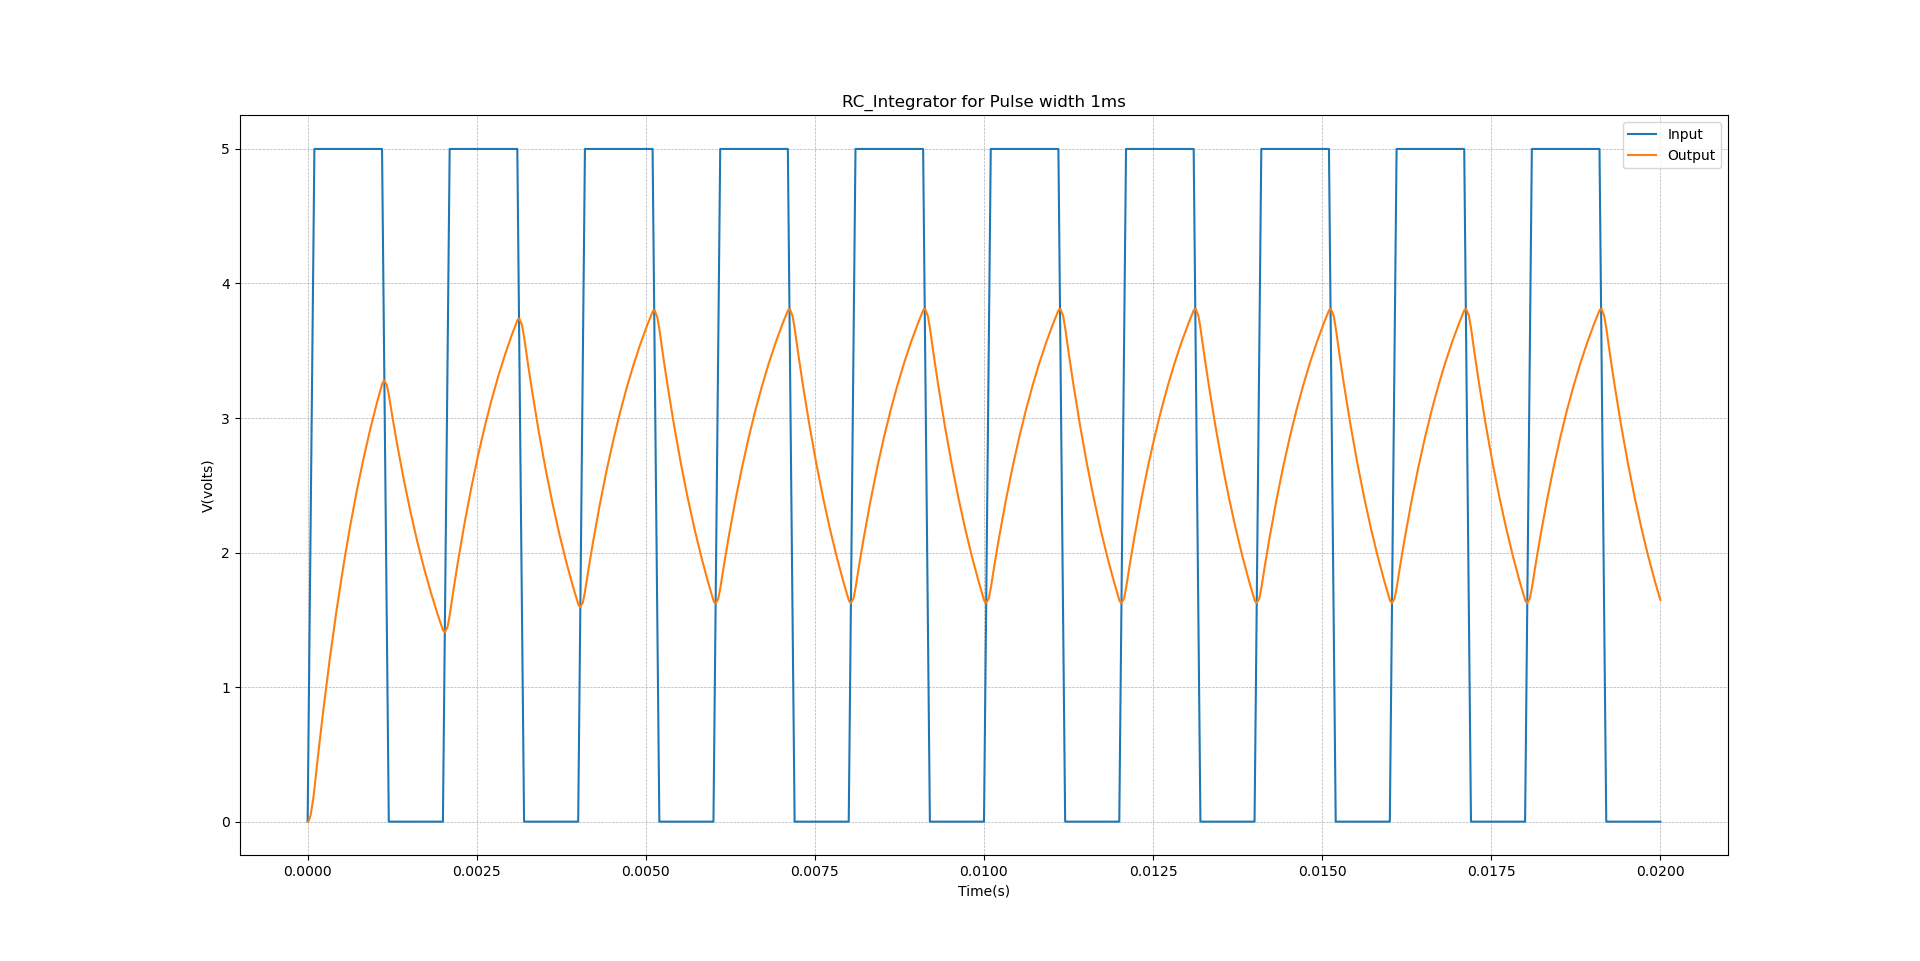
\includegraphics[width=\paperwidth]{RC_Integrator_3.png}}
\makebox[\textwidth]{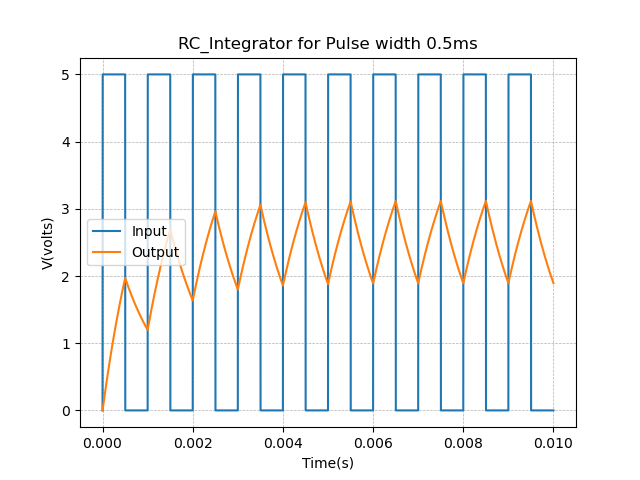
\includegraphics[width=\paperwidth]{RC_Integrator_4.png}}
\makebox[\textwidth]{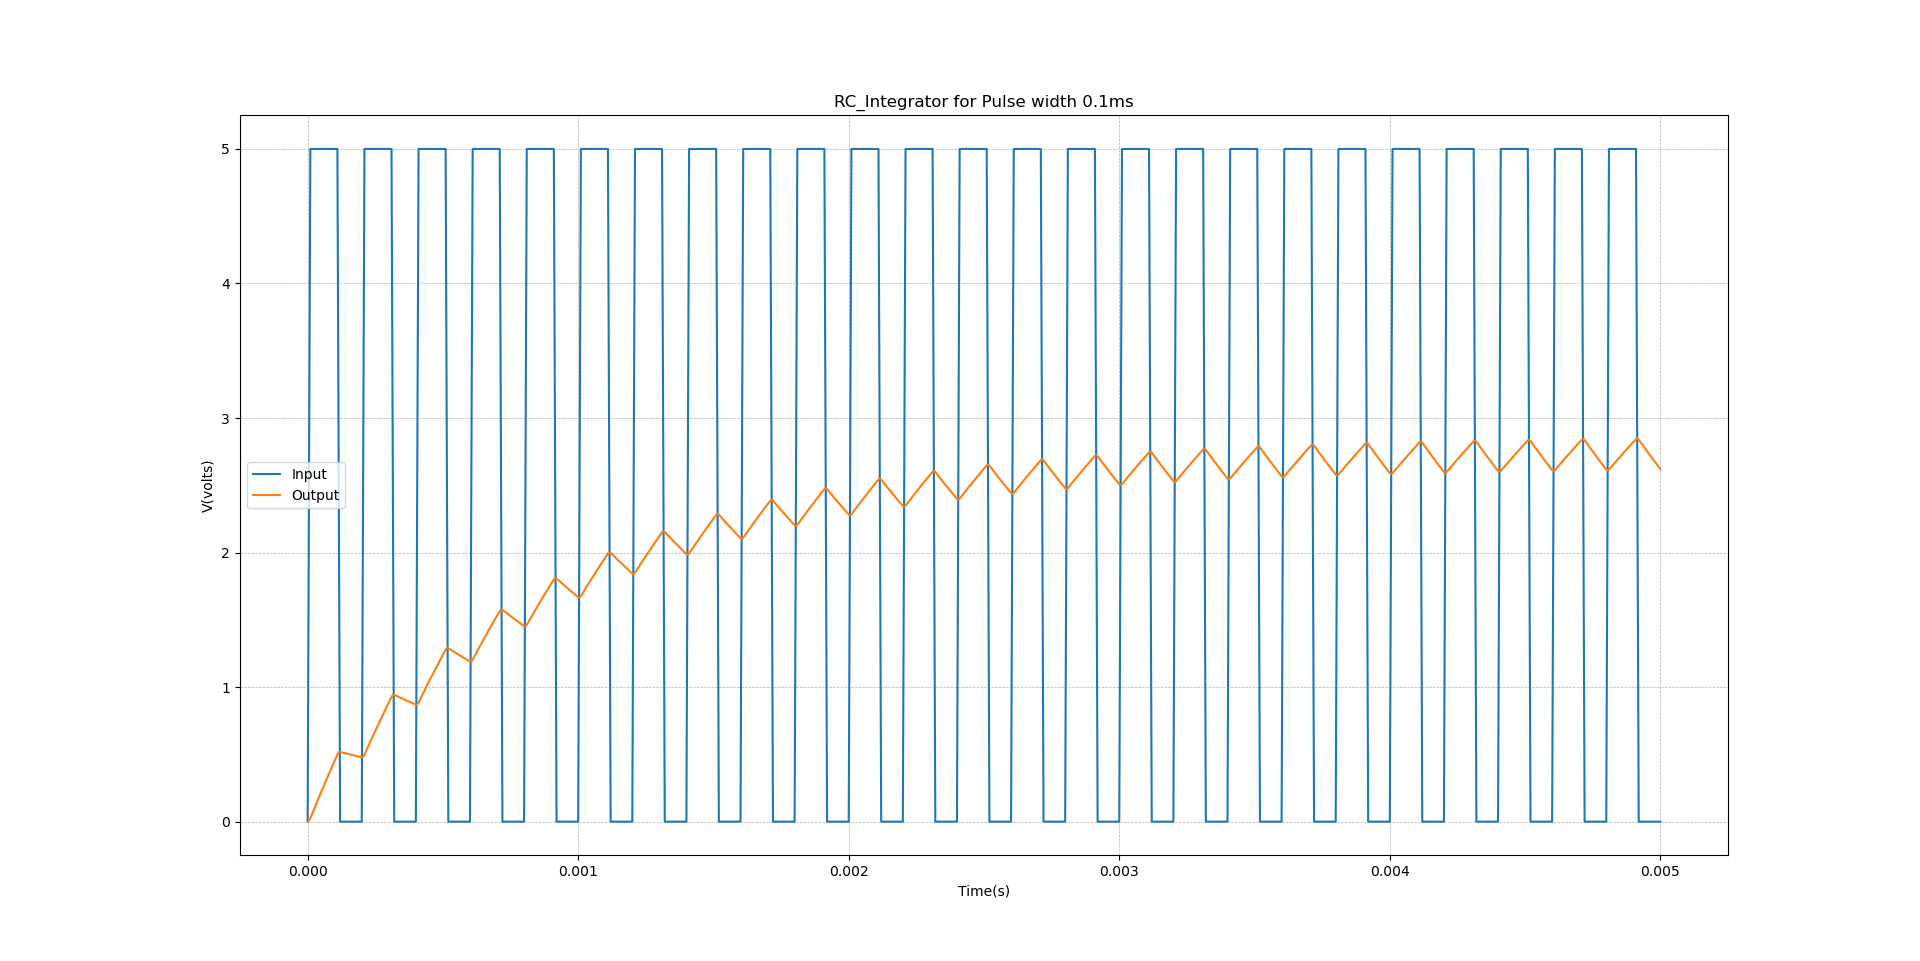
\includegraphics[width=\paperwidth]{RC_Integrator_5.png}}
\makebox[\textwidth]{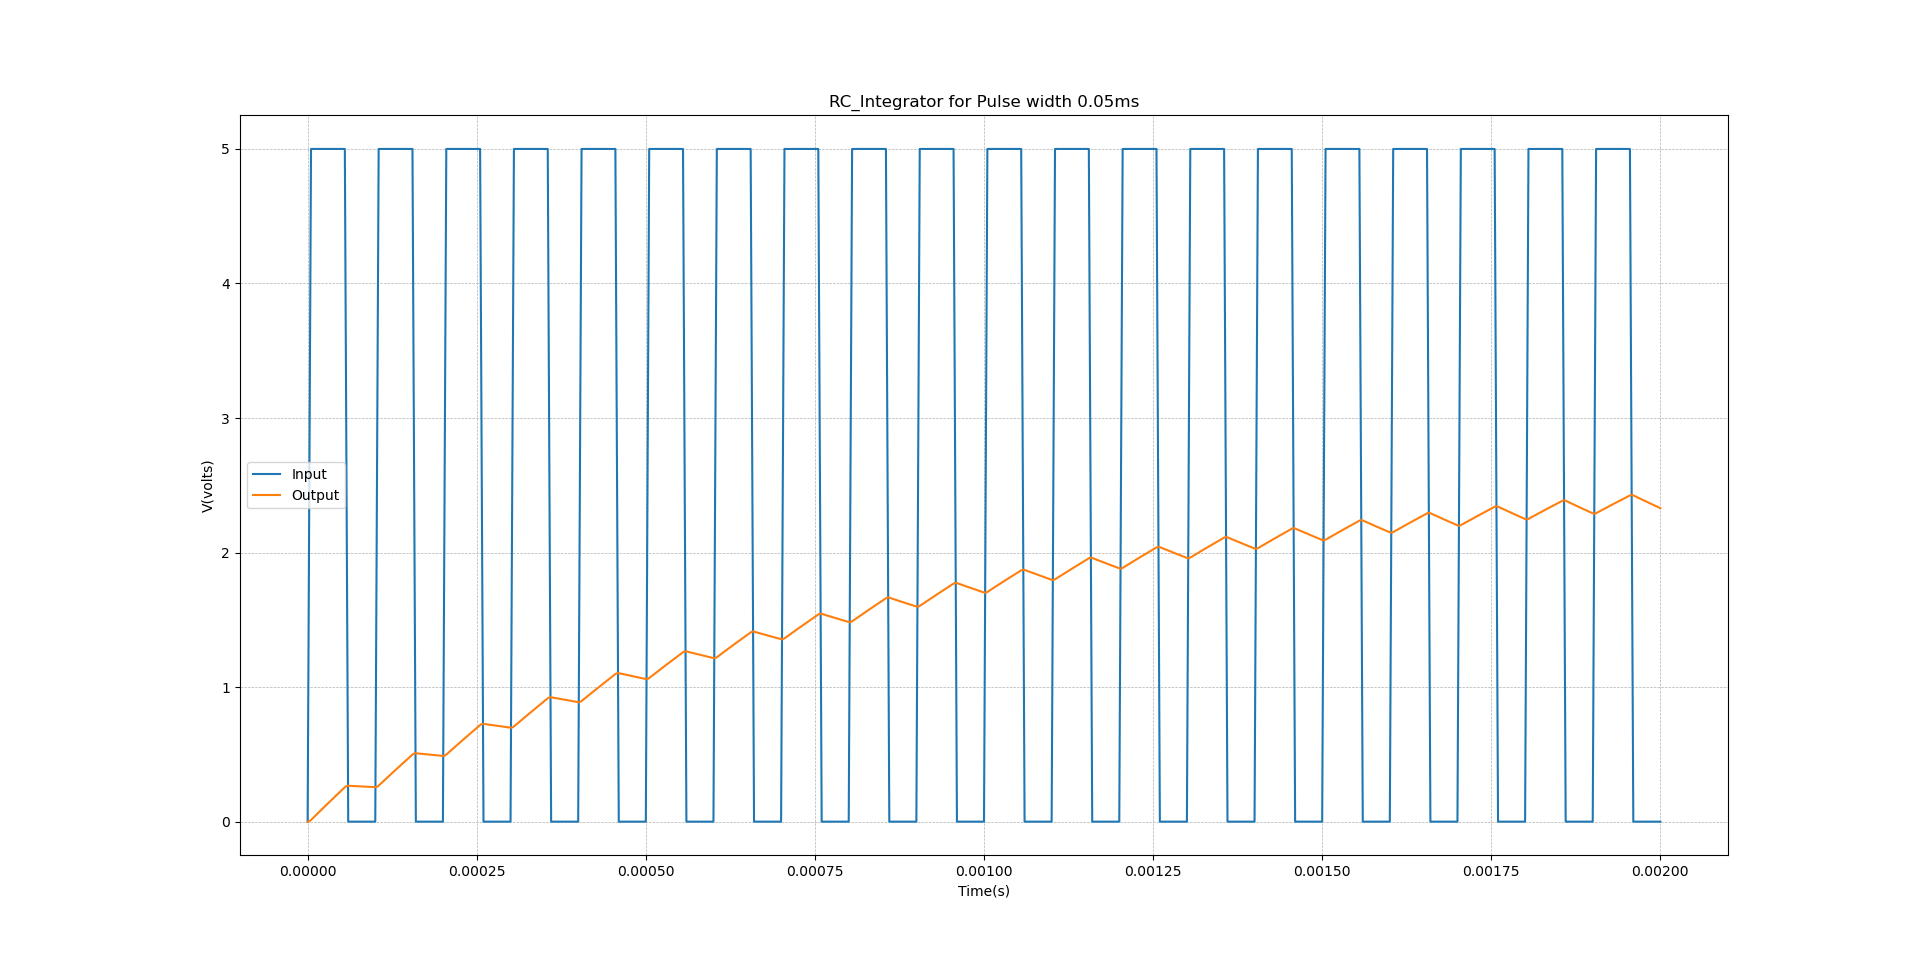
\includegraphics[width=\paperwidth]{RC_Integrator_6.png}}

\subsection{RC Differentiator}
\subsubsection{Code snippet}
\lstinputlisting{../RC_Differentiator.cir}
\subsubsection{Simulation results}
\makebox[\textwidth]{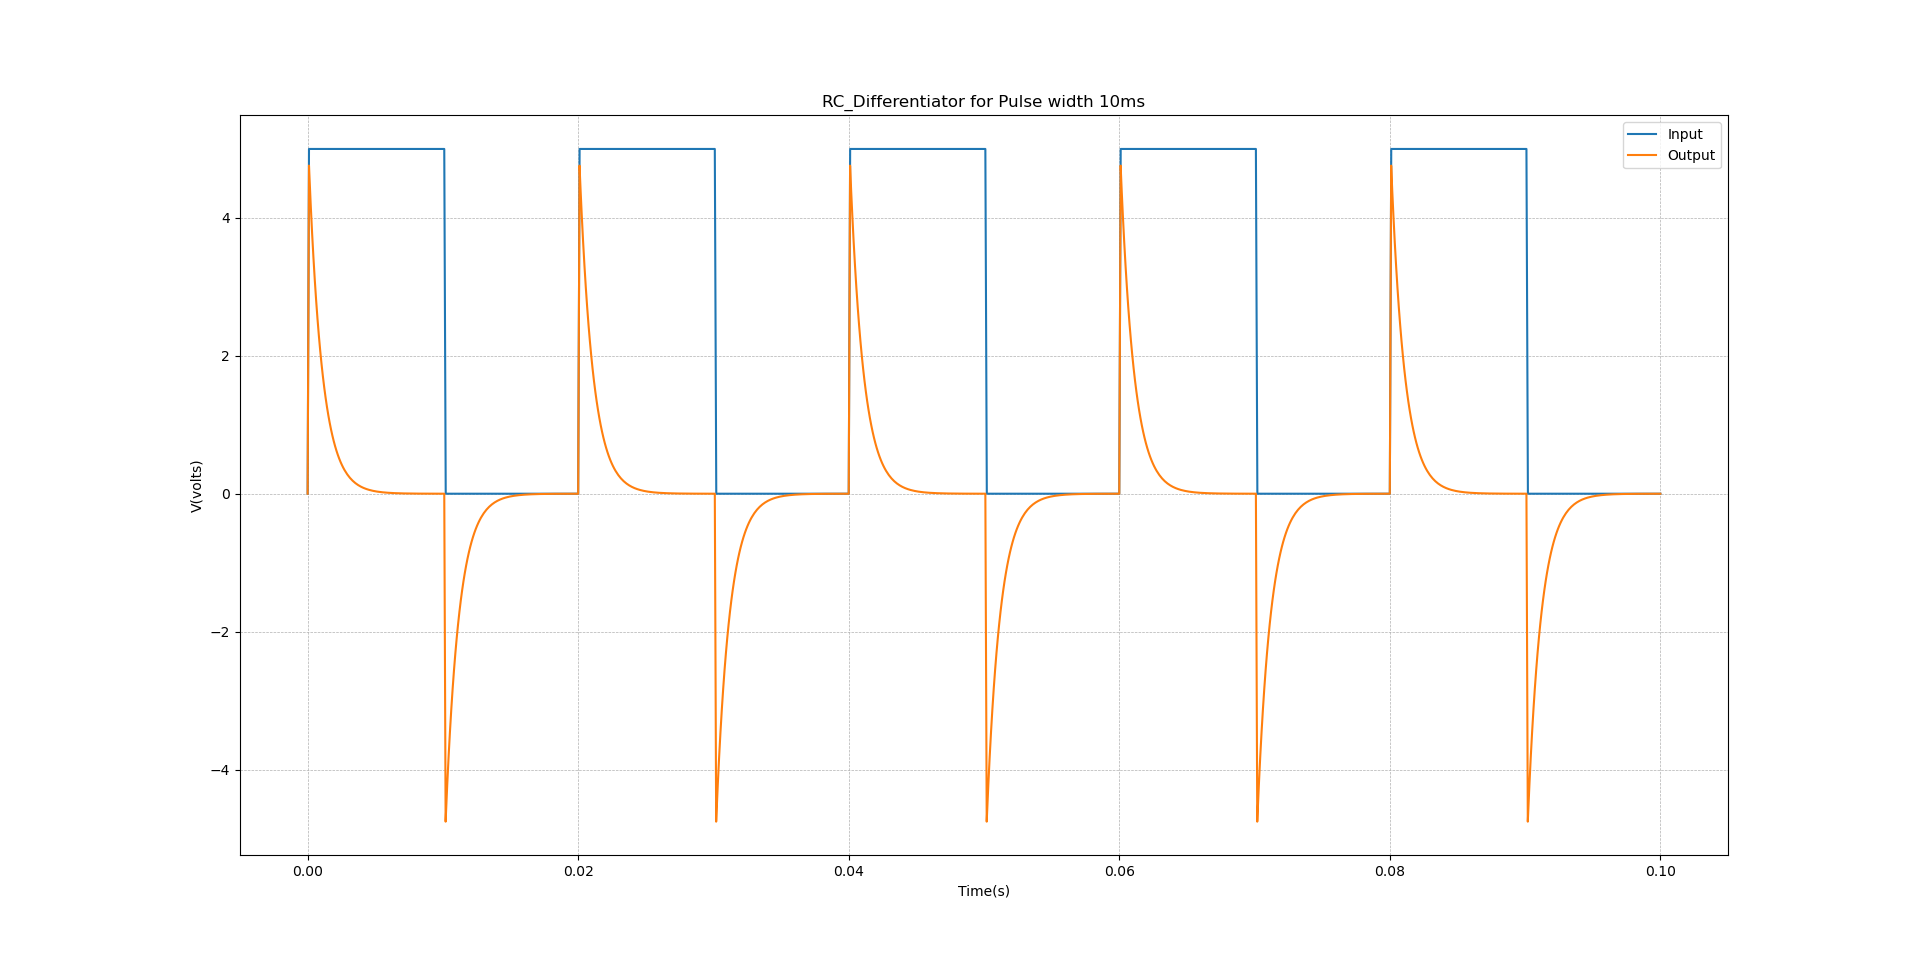
\includegraphics[width=\paperwidth]{RC_Differentiator_1.png}}
\makebox[\textwidth]{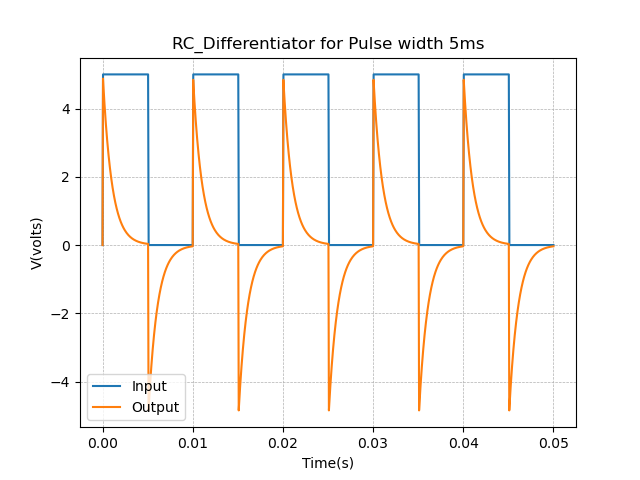
\includegraphics[width=\paperwidth]{RC_Differentiator_2.png}}
\makebox[\textwidth]{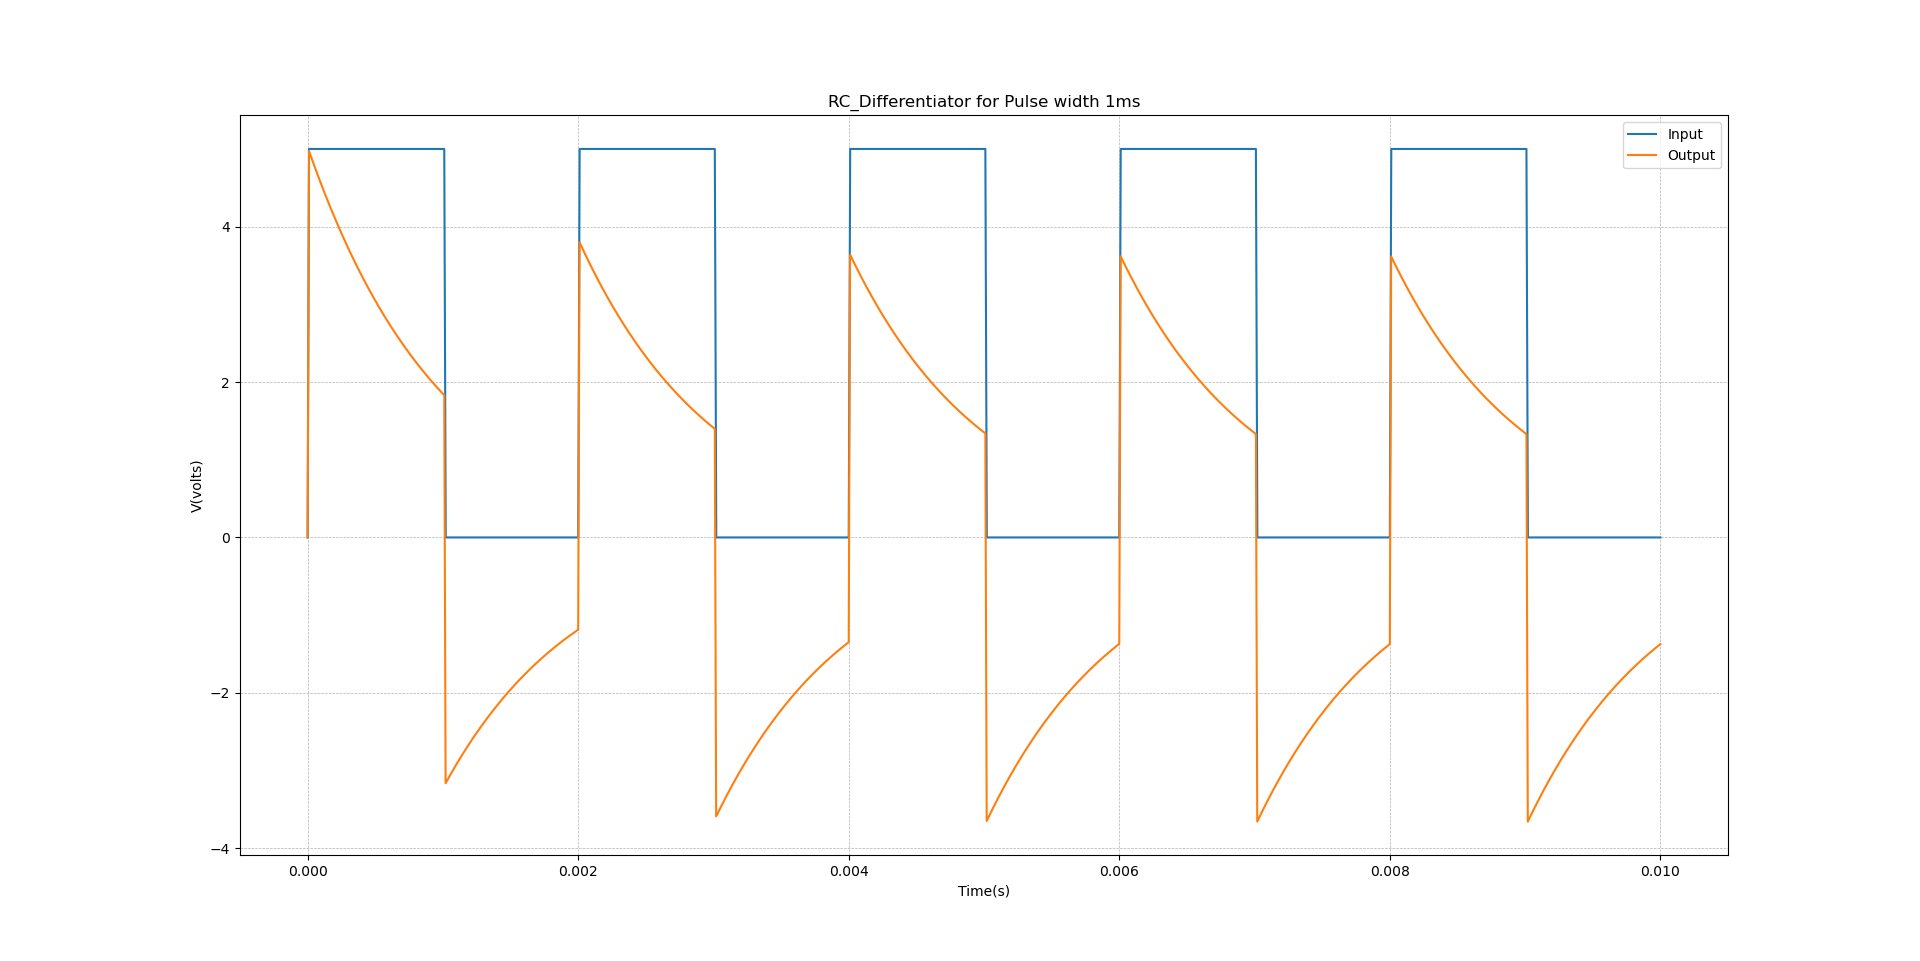
\includegraphics[width=\paperwidth]{RC_Differentiator_3.png}}
\makebox[\textwidth]{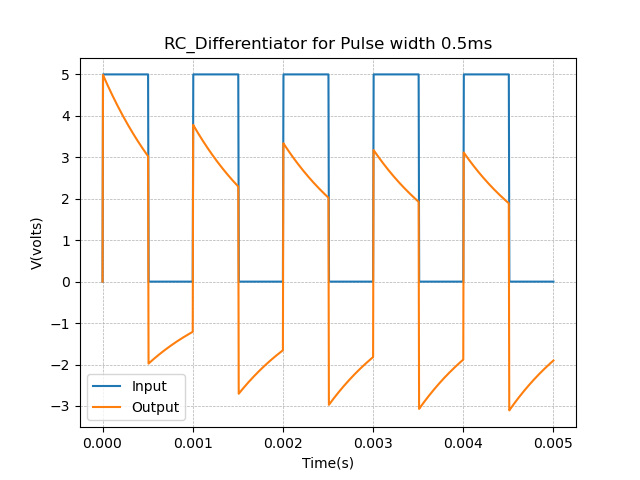
\includegraphics[width=\paperwidth]{RC_Differentiator_4.png}}
\makebox[\textwidth]{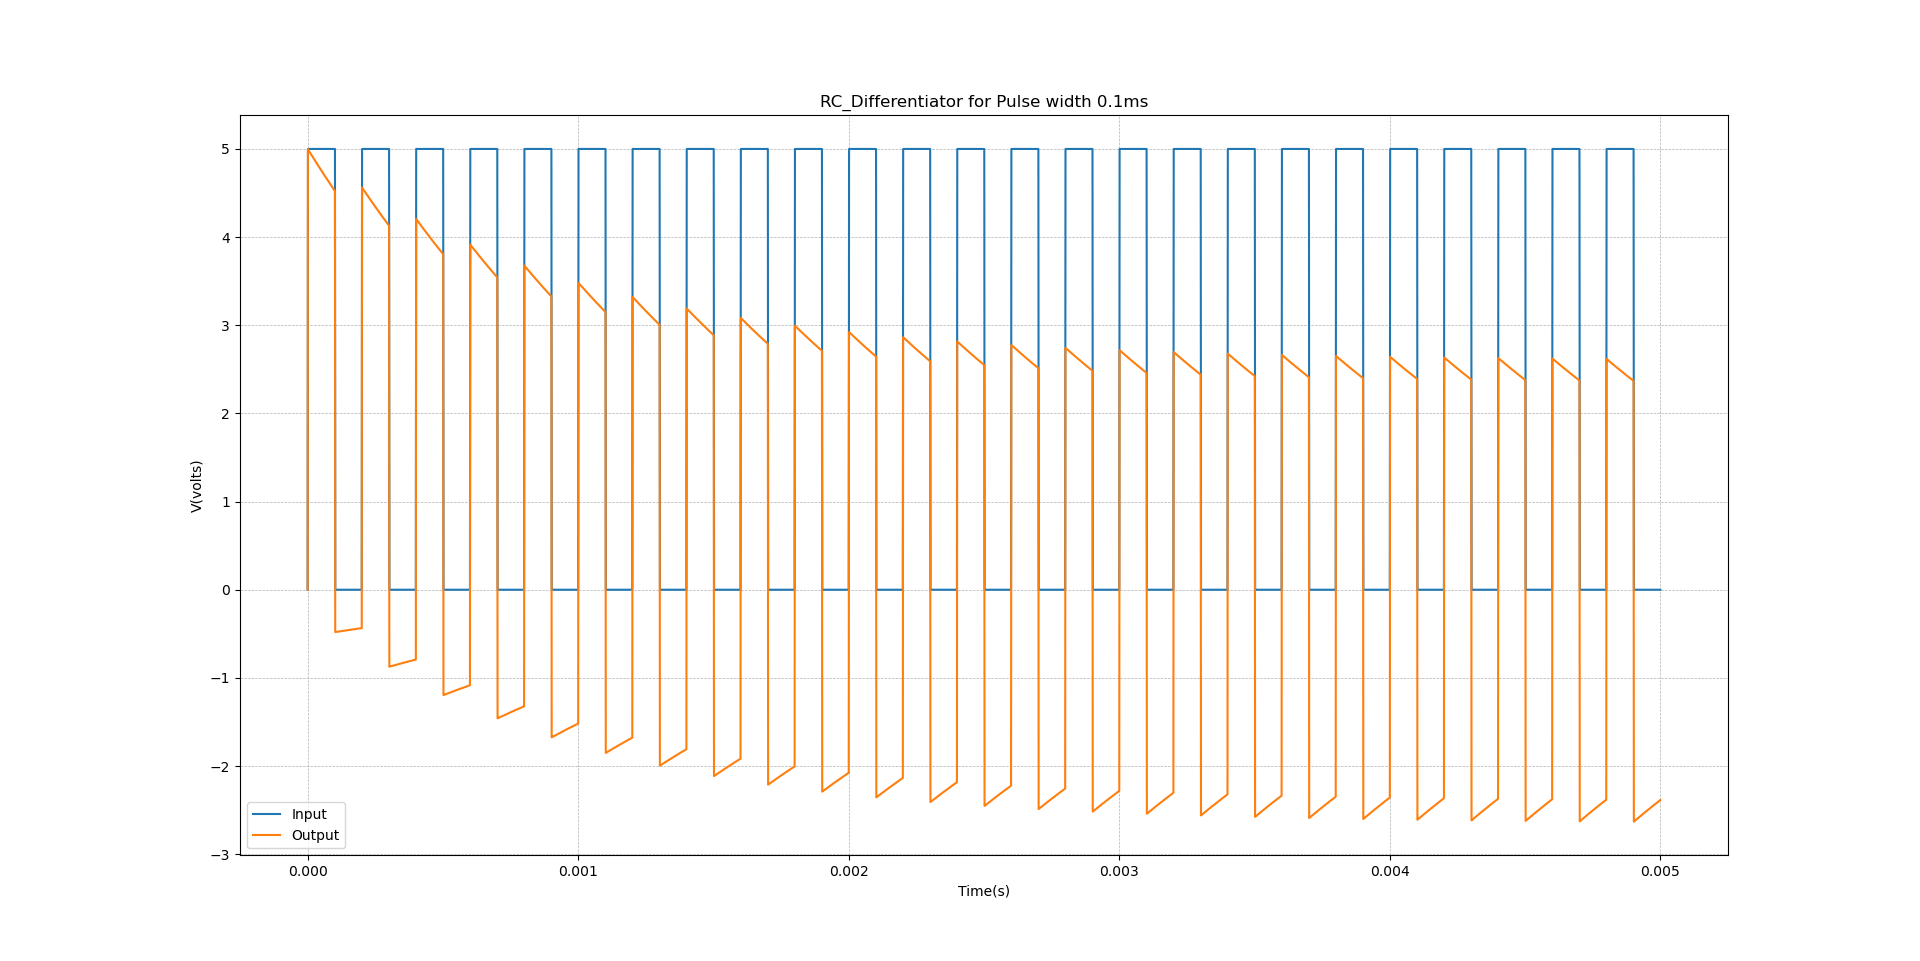
\includegraphics[width=\paperwidth]{RC_Differentiator_5.png}}
\makebox[\textwidth]{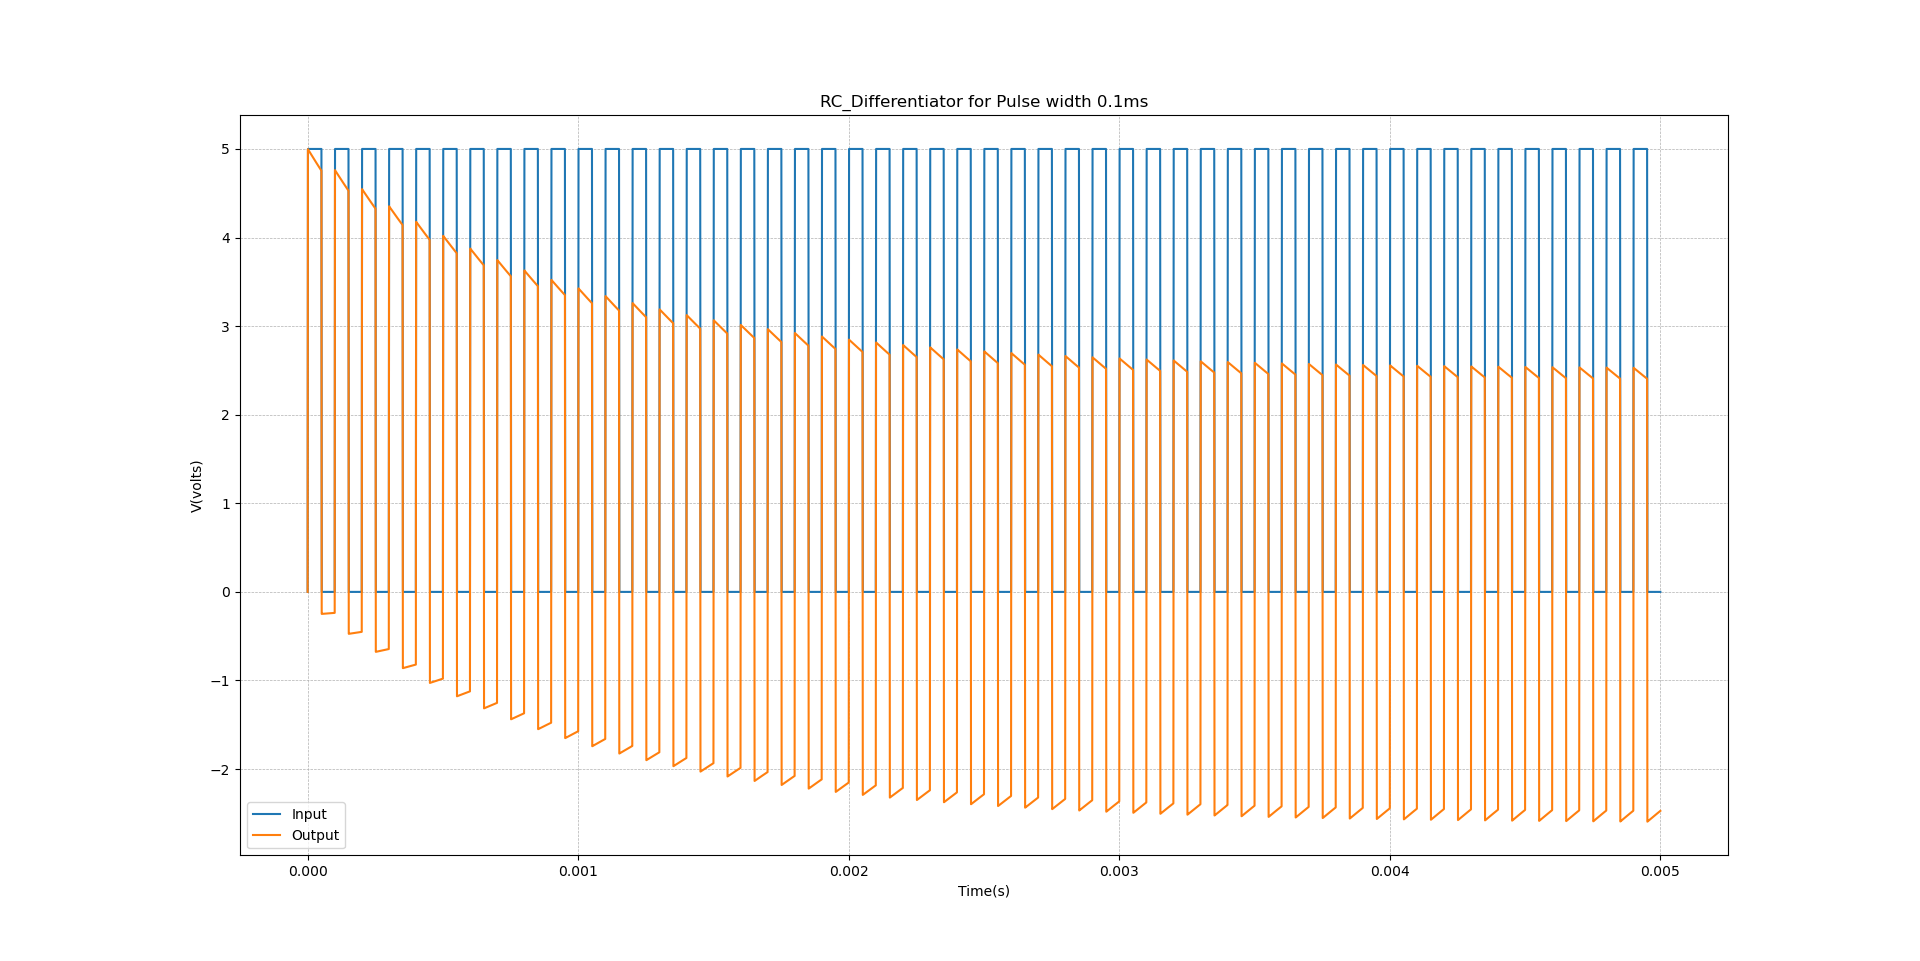
\includegraphics[width=\paperwidth]{RC_Differentiator_6.png}}

\subsection{RC Lowpass Filter}
\subsubsection{Code snippet}
\lstinputlisting{../RC_Lowpass_Filter.cir}
\subsubsection{Simulation results}
\makebox[\textwidth]{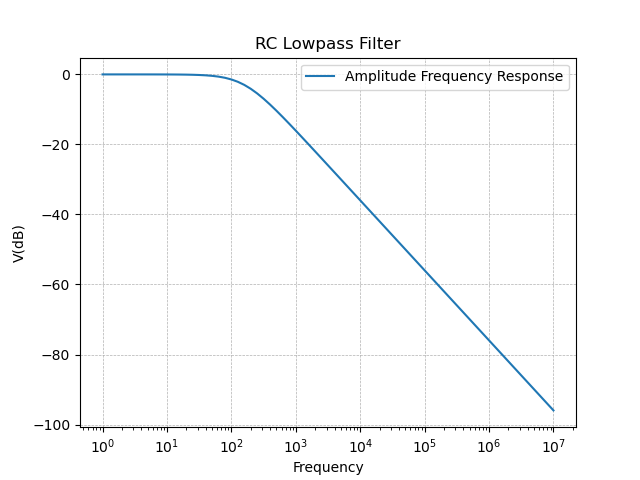
\includegraphics[width=\paperwidth]{RC_Lowpass_Filter.png}}

\subsection{RC Highpass Filter}
\subsubsection{Code snippet}
\lstinputlisting{../RC_Highpass_Filter.cir}
\subsubsection{Simulation results}
\makebox[\textwidth]{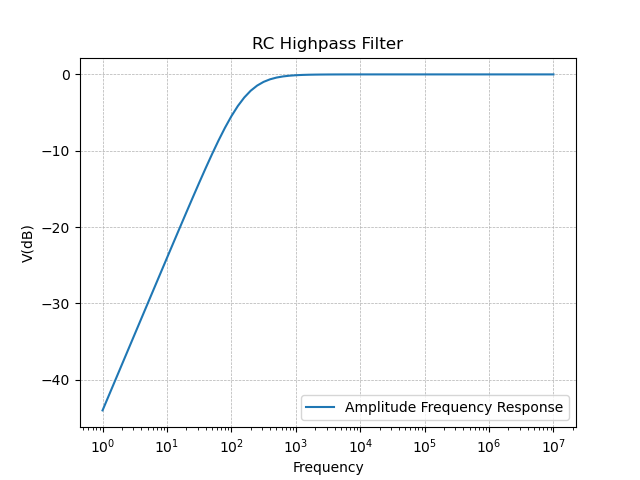
\includegraphics[width=\paperwidth]{RC_Highpass_Filter.png}}

\subsection{RC Bandpass Filter}
\subsubsection{Code snippet}
\lstinputlisting{../RC_Bandpass_Filter.cir}
\subsubsection{Simulation results}
\makebox[\textwidth]{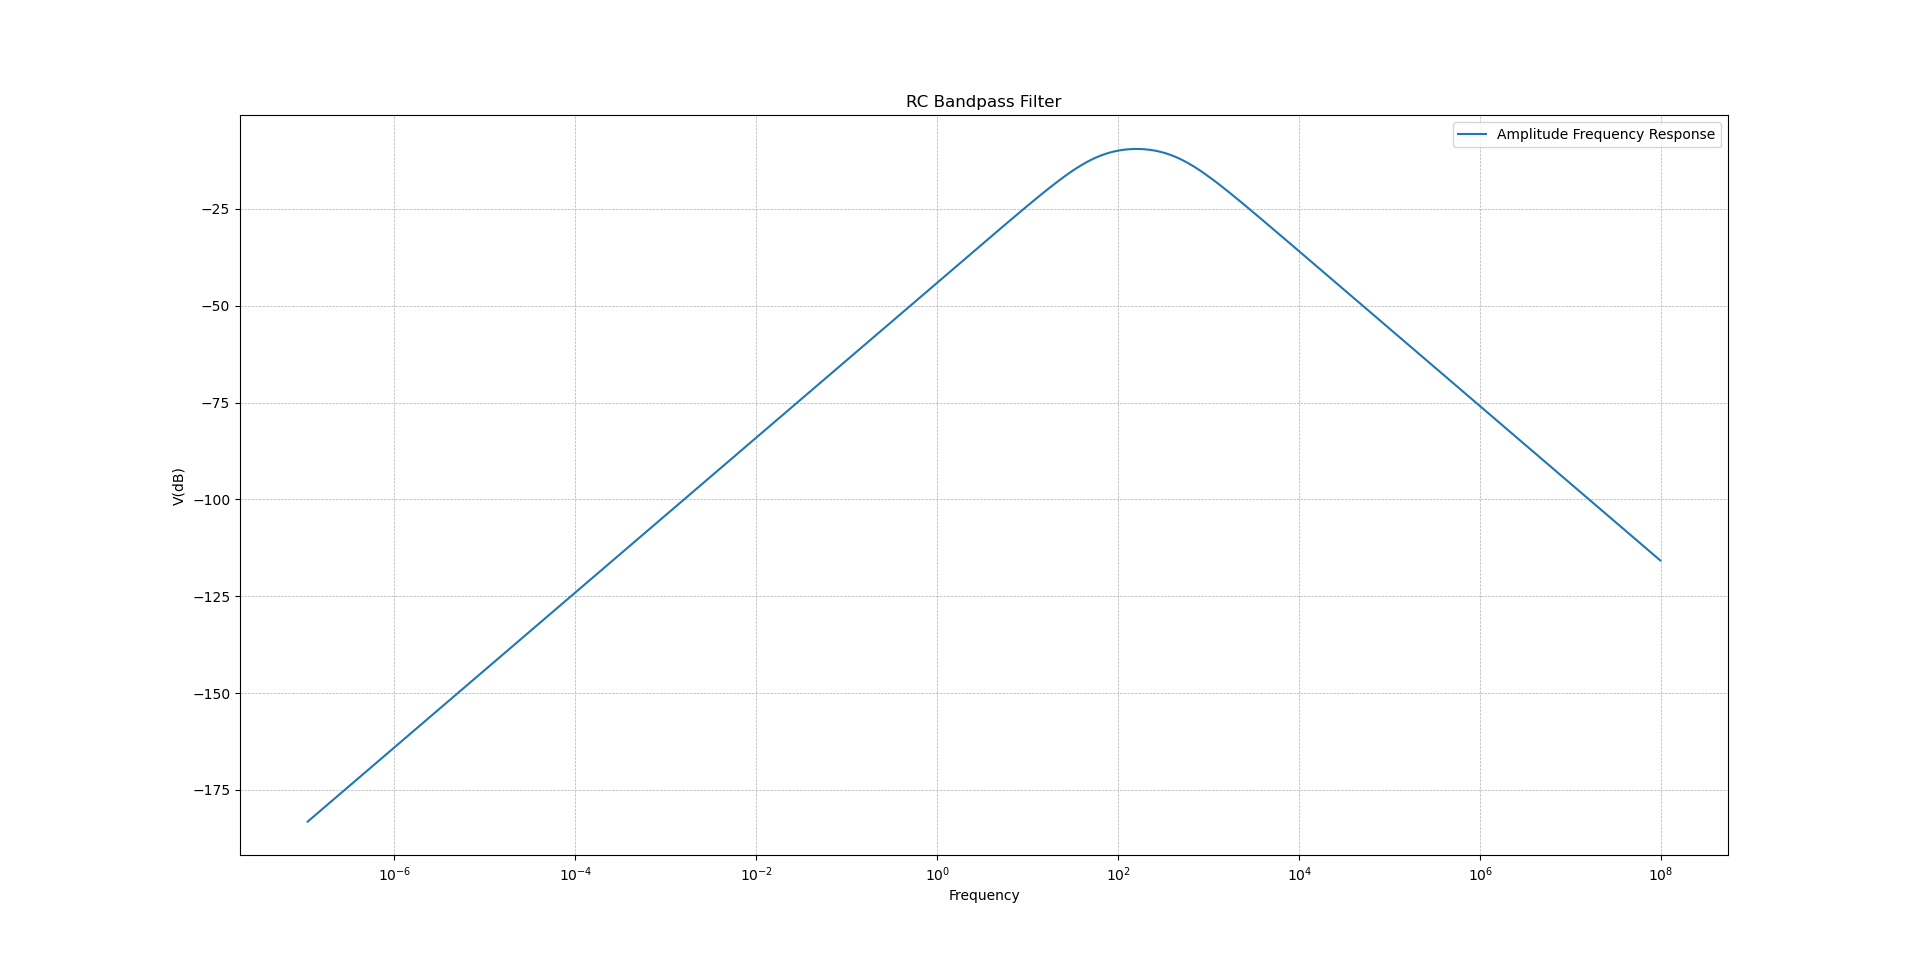
\includegraphics[width=\paperwidth]{RC_Bandpass_Filter.png}}

\subsection{RLC Bandpass Filter}
\subsubsection{Code snippet}
\lstinputlisting{../RLC_Bandpass_Filter.cir}
\subsubsection{Simulation results}
\makebox[\textwidth]{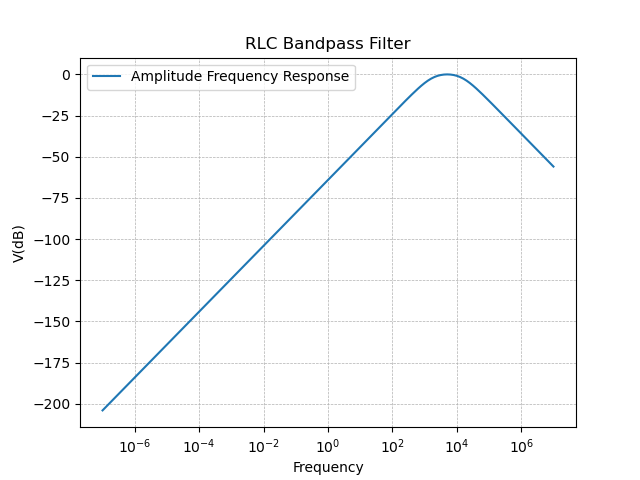
\includegraphics[width=\paperwidth]{RLC_Bandpass_FiIter.png}}


\section{Experimental results}

\subsection{RC Integrator}
\subsection{RC Differentiator}
\subsection{RC Lowpass Filter}
\subsection{RC Highpass Filter}
\subsection{RC Bandpass Filter}
\subsection{RLC Bandpass Filter}
\section{Experiment completion status}
All the sections were completed
\end{document}
